\begin{frame}{some constant time ideas}
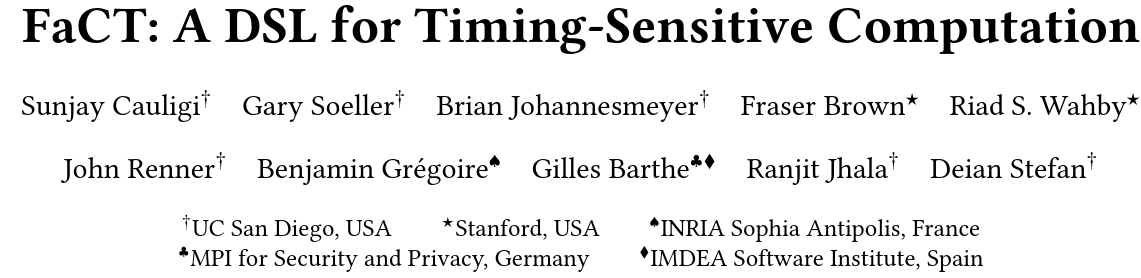
\includegraphics[width=0.8\textwidth]{../betterpl/fact-title}
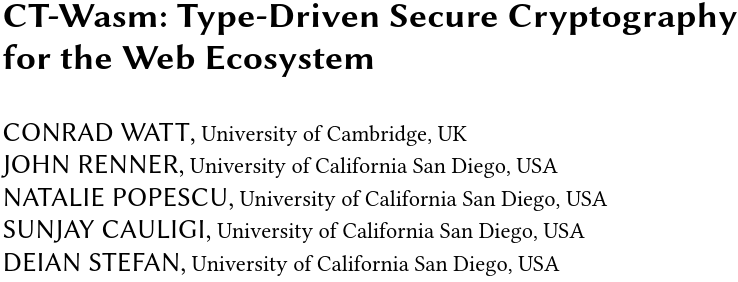
\includegraphics[width=0.8\textwidth]{../betterpl/ct-wasm-title}
\begin{itemize}
\item FaCT, PLDI 2019; CT-Wasm: POPL 2019
\end{itemize}
\end{frame}

\begin{frame}{constant-time programming languages}
    \begin{itemize}
    \item active research area, no consensus on what works best
    \vspace{.5cm}
    \item common approach: separate type for \textbf{secret} data
    \item compiler or language virtual machine disallows variable-time operations using secret data
    \item no secret-based array lookup (cache timing varies)
        \begin{itemize}
        \item e.g. array[secret\_value] $\rightarrow$ compile error (type mismatch)
        \end{itemize}
    \item no secret-based integer division (usually variable speed instruction)
    \item \ldots
    \vspace{.5cm}
    \item explicit operations for any secret-to-non-secret conversions
    \end{itemize}
\end{frame}
